% -------------------------------------------------------------------
\documentclass[usepdftitle=false,9pt]{beamer}

% Specify the respective Beamer theme here:
%\usetheme[height=0.3cm,width=1.8cm,shadow=false]{iue}


%encodings
\usepackage[utf8]{inputenc}
\usepackage[OT1]{fontenc}

%some useful packages
\usepackage[]{mathrsfs}
\usepackage[]{amssymb}
\usepackage[]{amsmath}
\usepackage[]{acronym}
\usepackage[]{listings}
\usepackage[]{xcolor}
\usepackage[]{graphicx}
\usepackage[]{textcomp} %for tilde
\usepackage{tikz}

\hypersetup{pdftitle = {PETSc - Portable, Extensible Toolkit for Scientific Computation}, pdfauthor={Karl Rupp (based on slides by Jed Brown et al.)}}


%% Listings package START
\usepackage{color}
\usepackage{listings}

\definecolor{darkblue}{rgb}{0,0,.6}
\definecolor{darkred}{rgb}{.6,0,0}
\definecolor{darkgreen}{rgb}{0,.6,0}
\definecolor{red}{rgb}{.98,0,0}
\definecolor{lightgrey}{rgb}{0.98,0.98,0.98}


\lstloadlanguages{C++}
\lstset{%
  language=C++,
  basicstyle=\small\ttfamily,
  commentstyle=\itshape\color{darkgreen},
  keywordstyle=\bfseries\color{darkblue},
  stringstyle=\color{darkred},
  showspaces=false,
  showtabs=false,
  columns=fixed,
  backgroundcolor=\color{lightgrey},
  numbers=none,
  frame=single,
  numberstyle=\tiny,
  breaklines=true,
  showstringspaces=false,
  xleftmargin=0.1cm,
  xrightmargin=3em
}%

\lstset{emphstyle=\color{red}}

%% Listings package STOP








\renewcommand{\matrix}[1]{\boldsymbol{#1}}
\renewcommand{\vector}[1]{\boldsymbol{#1}}
\renewcommand{\d}{\mathrm{d}}
\newcommand{\domelem}[1]{\boldsymbol{\mathrm{#1}}}
\newcommand{\kB}{k_\mathrm{B}}
\newcommand{\VT}{V_\mathrm{T}}
\newcommand{\q}{\mathrm{q}}
\newcommand{\LandauO}{\mathcal{O}}
\newcommand{\Bullet}{$\triangleright$}
\newcommand{\black}{ }
\newcommand{\ViennaCL}{\texttt{ViennaCL}}

%\setlength{\fboxrule}{1pt}

%\renewcommand{\seriesdefault}{\bfdefault}
%\usepackage{helvet}

\graphicspath{{figures/}}           % in which folder all the figures are
\newcommand{\tn}   {\textnormal}

%\mode<presentation>

% table of contents, depth
\setcounter{tocdepth}{2}

% modify at will
\setbeamercovered{transparent}


\author[Karl Rupp]{Karl Rupp \\ \ttfamily rupp@mcs.anl.gov}

\institute[ANL]
{ \footnotesize
  Mathematics and Computer Science Division \\
  Argonne National Laboratory \\
}

\title[PETSc]{ { \Huge PETSc } \\[0.5em] Portable, Extensible Toolkit for Scientific Computation}

\date[HPC Symposium, April 10th, 2013]{ \footnotesize Tutorial at the HPC Symposium 2013 \\[2em] April 10th, 2013}

\setbeamertemplate{blocks}[default]
%\setbeamercolor{block title}{bg=}
\setbeamercolor{block body}{bg=}
\setbeamercovered{transparent}

\begin{document}

\begin{frame}[plain]
 \frametitle{~}
 \titlepage
\end{frame}







% \begin{frame}{Who is this Guy?}
% 
%  \begin{center}
%    \includegraphics[width=0.6\textwidth]{figures/who-is-this-guy} \\
%  \scriptsize http://memeshappen.com/media/created/-WHO-IS-THIS-GUY--meme-55268.jpg
%  \end{center}
% 
% \end{frame}


\begin{frame}{Introduction}

 \begin{minipage}{0.68\textwidth}
 \begin{block}{Positions}
   \begin{itemize}
    \item PhD student at TU Wien (2009-2011)
    \item Postdoc at Argonne Natl.~Lab.~(09/2012-09/2013)
    \item Postdoc at TU Wien (09/2013-10/2015; 01/2017-)
    \item Freelancer, ETH Z\"urich (03/2016-06/2017)
   \end{itemize}
 \end{block}

 \begin{block}{Research Interests}
   \begin{itemize}
    \item Numerical solution of PDEs
    \item Semiconductor device simulation
    \item Parallel computing
   \end{itemize}
 \end{block}

 \begin{block}{Software Development}
   \begin{itemize}
    \item PETSc
    \item ViennaCL
    \item ViennaSHE
    \item ...
   \end{itemize}
 \end{block}
 \end{minipage}
  \begin{minipage}{0.3\textwidth}
%  \includegraphics[width=0.99\textwidth]{figures/kangaroos-austria}
 \end{minipage}

\end{frame}



%%
%% Introduction
%%


\begin{frame}[fragile]{Matrix Multiplication}

  \begin{block}{Dense Matrix-Matrix-Multiplications}
  \begin{itemize}
   \item Ubiquituous for: dense linear algebra (eigenvalues, LU factorization, etc.)
   \item FLOP-limited, basis for TOP500
   \item Computer scientist's darling
  \end{itemize}
 \end{block}


 \begin{center}
   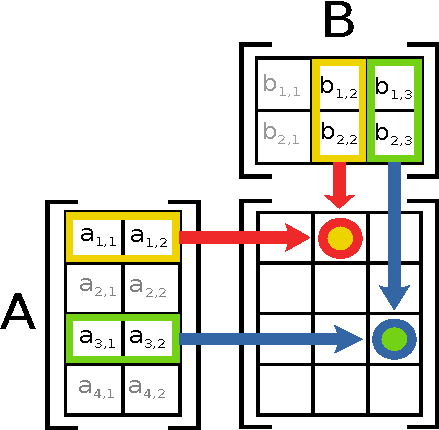
\includegraphics[width=0.4\textwidth]{figures/gemm_diagram_2} \\
 \tiny \verb|https://en.wikipedia.org/wiki/Matrix_multiplication#/media/File:Matrix_multiplication_diagram_2.svg|
 \end{center}

\end{frame}



% \begin{frame}{Why Sparse Matrices?}
% 
%  \begin{minipage}{0.5\textwidth}
%   \includegraphics[width=0.99\textwidth]{figures/social-graph.jpg}
%  \end{minipage} \hfill \pause
%  \begin{minipage}{0.45\textwidth}
%   \begin{align*}
%    \left(
%    \begin{array}{ccccccccc}
%     1 & 1 & 1 & 0 &  & 0 & 0 & 0 & 0 \\
%     0 & 1 & 1 & 0 &  & 0 & 0 & 0 & 0 \\
%     1 & 1 & 1 & 1 &  & 1 & 0 & 0 & 0 \\
%     0 & 0 & 1 & 1 &  & 0 & 0 & 0 & 0 \\
% & \\
%     0 & 0 & 1 & 0 &  & 1 & 1 & 1 & 1 \\
%     0 & 0 & 0 & 0 &  & 1 & 1 & 0 & 0 \\
%     0 & 0 & 0 & 0 &  & 1 & 0 & 1 & 0 \\
%     0 & 0 & 0 & 0 &  & 1 & 0 & 0 & 1 \\
%     \end{array}
%    \right)
%   \end{align*}
%  \end{minipage}
%  
%  \pause
%  
%  \vspace*{1cm}
%  \begin{center}
%   Distance-2 connectivity given by the squared matrix \\
%   \pause
%   ...\\
%   Distance-$n$ connectivity given by the $n$-th power \\
%  \end{center}
%  \vspace*{-1cm}
% 
% 
% \end{frame}


% 
% \begin{frame}{Why Sparse Matrices?}
% 
% \begin{center}
%  \begin{center}
%    \includegraphics[width=0.9\textwidth]{figures/multigridgrid} \\
%  \scriptsize http://web.utk.edu/~wfeng1/style/mggrid.png
%  \end{center}
% \end{center}
% \end{frame}
% 


% 
% \begin{frame}{Why Sparse Matrices?}
% 
%  \begin{block}{Sparse Matrices}
%   \begin{itemize}
%    \item Ubiquituous for: graph algorithms, numerical solution of PDEs
%    \item Finite differences, finite elements, finite volumes, etc.
%   \end{itemize}
%  \end{block}
% 
%  \begin{block}{Algebraic Multigrid}
%   \begin{itemize}
%    \item Asymptotically optimal solver
%    %\item Construct coarse grid hierarchy from matrix entries only
%    \item Computation of coarse grid operator $\mathbf{A}^{\mathrm{coarse}} = \mathbf{R} \mathbf{A}^{\mathrm{fine}} \mathbf{P}$ expensive
%    %\item Sparse Matrix Products are the performance bottleneck
%   \end{itemize}
%  \end{block}
% 
%  \begin{center}
%   \includegraphics[width=0.6\textwidth]{figures/smooth-error.png} \\
%   \scriptsize https://str.llnl.gov/str/December03/gifs/falgout2.jpg
%  \end{center}
% 
% \end{frame}
% 
% 
% 
% \begin{frame}{Why Sparse Matrices?}
% 
% \begin{center}
%  \begin{center}
%    \includegraphics[width=0.95\textwidth]{figures/two-grid-smoothing.png} \\
%  \scriptsize [A.~Al Jarro, A.~Clo,H.~Bagci, 2012]
%  \end{center}
% \end{center}
% \end{frame}


\begin{frame}{Compressed Sparse Row Format}

 \begin{block}{Sparse Matrix Storage}
\begin{center}
 \begin{center}{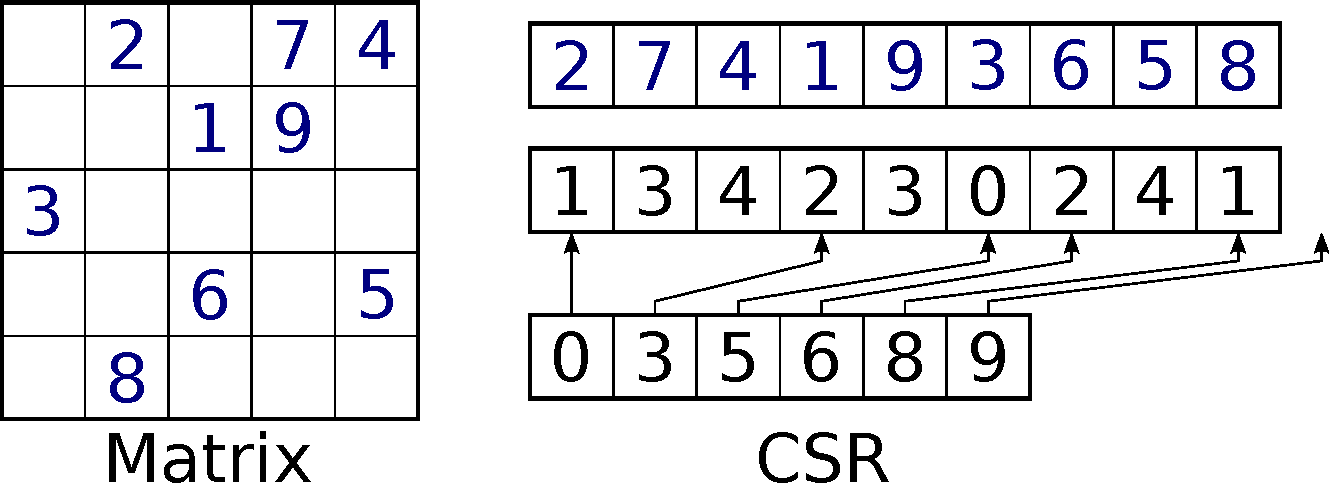
\includegraphics[height=40mm]{figures/matrix_csr}}\end{center}
\end{center}
 \end{block}


\end{frame}


%%
%% Explain basic principles of SpGEMM
%%



\begin{frame}{Sparse Matrix Products}

\begin{center}
 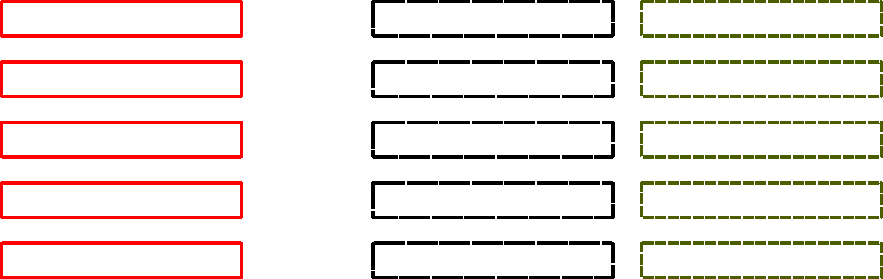
\includegraphics[width=0.85\textwidth]{figures/spgemm-matrix-1} \\
 \begin{align*}
  \qquad \mathbf{C} \qquad \qquad = \qquad \qquad \qquad \mathbf{A} \qquad \qquad \qquad \qquad \mathbf{B}
 \end{align*}
 \vspace*{-0.22cm}
\end{center}

\end{frame}


\begin{frame}{Sparse Matrix Products}

\begin{center}
 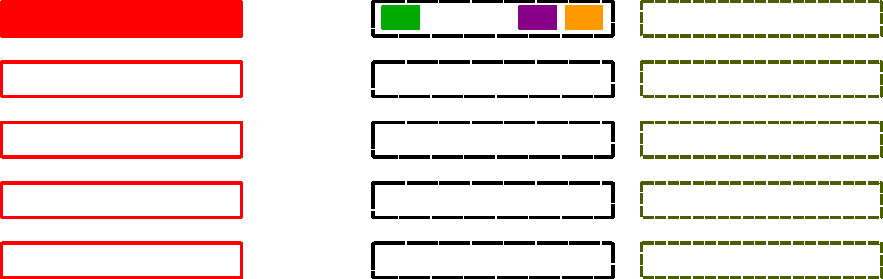
\includegraphics[width=0.85\textwidth]{figures/spgemm-matrix-2} \\
 \begin{align*}
  \mathrm{Row\ i:} \qquad \qquad \mathbf{c}_i \qquad \quad =\qquad \sum_{j} \qquad a_{ij} \qquad \qquad \qquad \mathbf{b}_j \qquad \qquad \qquad
 \end{align*}
\end{center}


\end{frame}

\begin{frame}{Sparse Matrix Products}

\begin{center}
 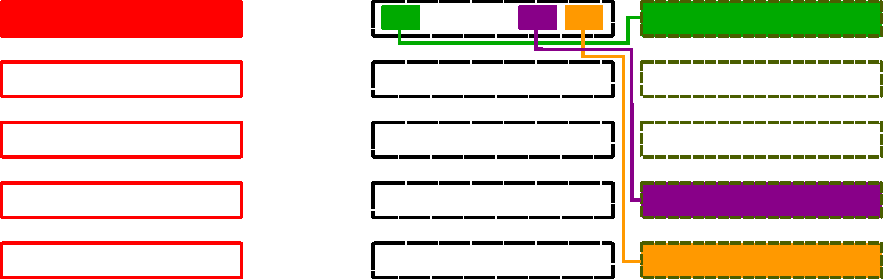
\includegraphics[width=0.85\textwidth]{figures/spgemm-matrix-3} \\
 \begin{align*}
  \mathrm{Row\ i:} \qquad \qquad \mathbf{c}_i \qquad \quad =\qquad \sum_{j} \qquad a_{ij} \qquad \qquad \qquad \mathbf{b}_j \qquad \qquad \qquad
 \end{align*}
\end{center}

\end{frame}

%%%%%%%%%%%


%%
%% Algorithms in PETSc
%%




\begin{frame}{Sparse Matrix-Matrix Multiplications}

 \begin{block}{Sequential MatMatMult in PETSc}
  \begin{itemize}
   \item Sorted
   \item Scalable
   \item Scalable, fast
   \item Heap
   \item BTHeap
   \item Linked-list condensed
   \item RowMerge -- {\color{red}NEW!}
   \item RowMerge2 -- {\color{red}NEW!}
  \end{itemize}
 \end{block}

 \pause
 \begin{block}{Two Stages}
  \begin{itemize}
   \item Symbolic phase: Determine sparsity pattern
   \item Numeric phase: Compute numerical values, sparsity pattern known
  \end{itemize}
 \end{block}

\end{frame}




\begin{frame}{Sparse Matrix-Matrix Multiplications}

 \begin{center}\Large \textbf{Good News:} \\[2em] %\includegraphics[width=0.6\textwidth]{figures/good-news}\\ {\tiny http://www.dsoconnections.org/wp-content/uploads/2017/05/Good-news-750x400.jpg}\\[2em]
                      \textbf{Numeric phase is easy!}\end{center}

\end{frame}


\begin{frame}{Sparse Matrix-Matrix Multiplications}

\begin{center}
\only<1>{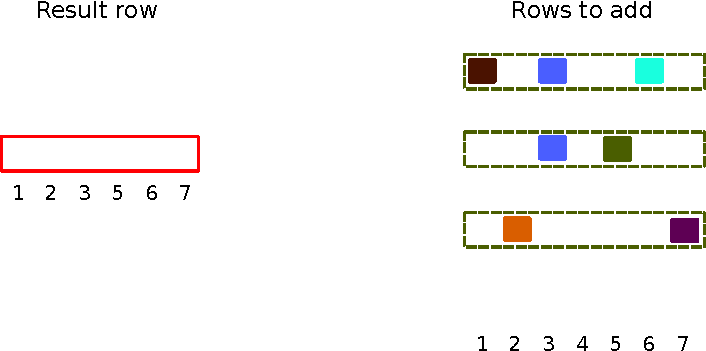
\includegraphics[width=0.7\textwidth]{figures/spgemm-numeric-1} }\only<2>{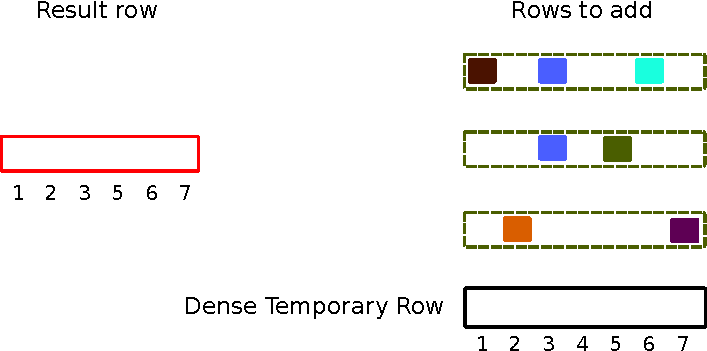
\includegraphics[width=0.7\textwidth]{figures/spgemm-numeric-2} }\only<3>{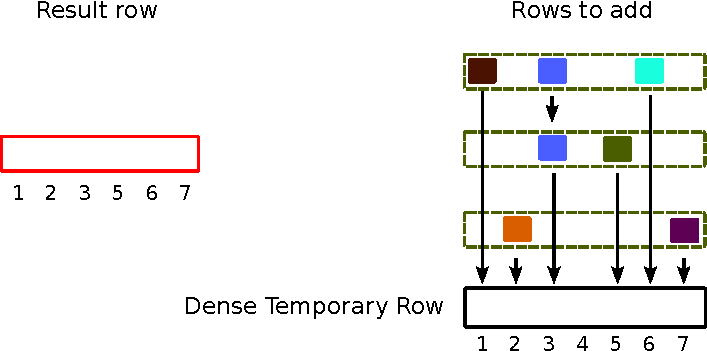
\includegraphics[width=0.7\textwidth]{figures/spgemm-numeric-3} }\only<4>{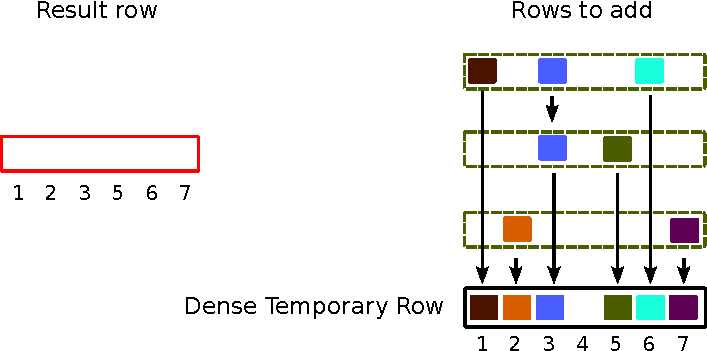
\includegraphics[width=0.7\textwidth]{figures/spgemm-numeric-4} }\only<5>{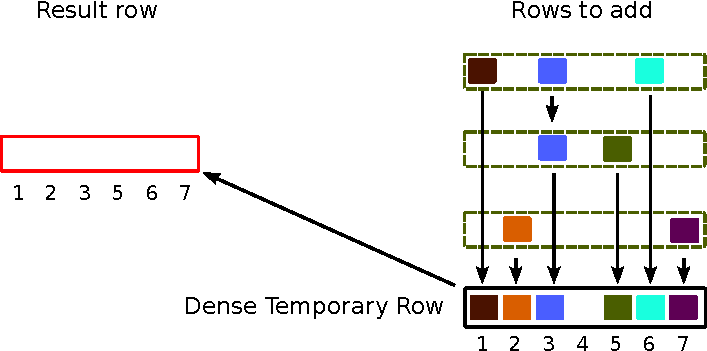
\includegraphics[width=0.7\textwidth]{figures/spgemm-numeric-5} }\only<6->{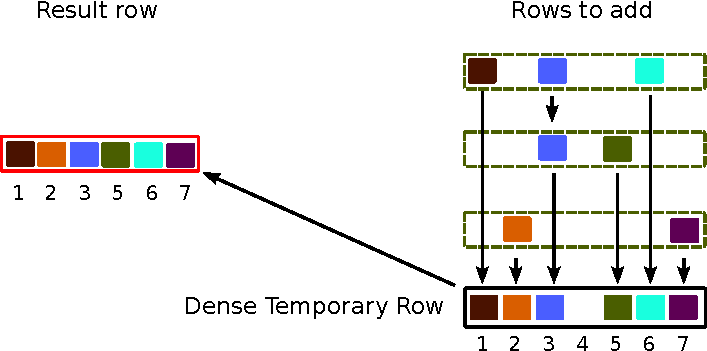
\includegraphics[width=0.7\textwidth]{figures/spgemm-numeric-6} }
\end{center}


 \begin{block}{Numeric Phase}
  \begin{itemize}
   \visible<2->{\item Merge directly to dense array}
   \visible<5->{\item Pick up nonzeros to form $\mathbf{C}$}
  \end{itemize}
 \end{block}

\end{frame}




\begin{frame}{Sparse Matrix-Matrix Multiplications}

 \begin{center}\Large \textbf{Bad News:} \\[2em] %\includegraphics[width=0.5\textwidth]{figures/bad-news}\\ {\tiny http://workingcapitalreview.com/wp-content/uploads/2015/03/20120802221109\_badnews.jpg}\\[2em]
                      \textbf{Symbolic phase is tricky!}\end{center}

\end{frame}





\begin{frame}{Sparse Matrix-Matrix Multiplications}

\begin{center}
\only<1>{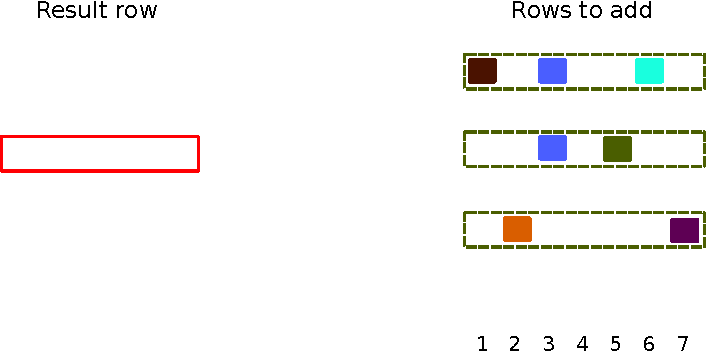
\includegraphics[width=0.7\textwidth]{figures/spgemm-sorted-1} }\only<2>{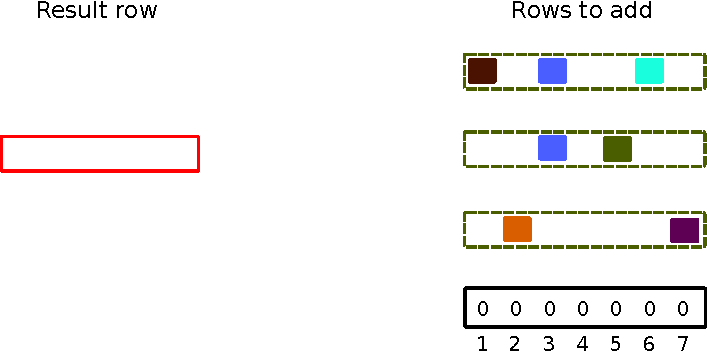
\includegraphics[width=0.7\textwidth]{figures/spgemm-sorted-2} }\only<3>{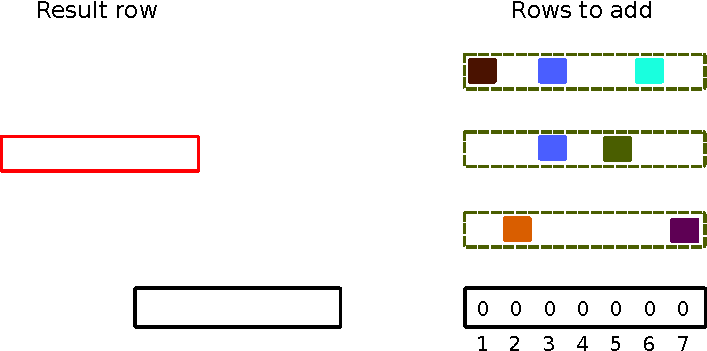
\includegraphics[width=0.7\textwidth]{figures/spgemm-sorted-3} }\only<4>{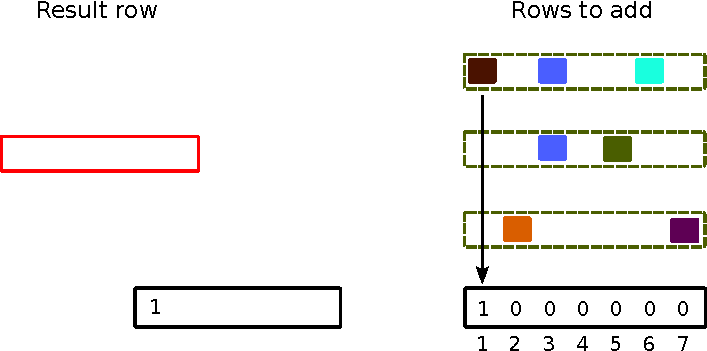
\includegraphics[width=0.7\textwidth]{figures/spgemm-sorted-4} }\only<5>{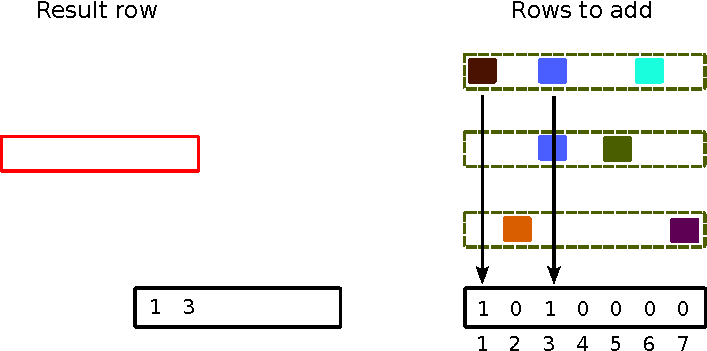
\includegraphics[width=0.7\textwidth]{figures/spgemm-sorted-5} }\only<6>{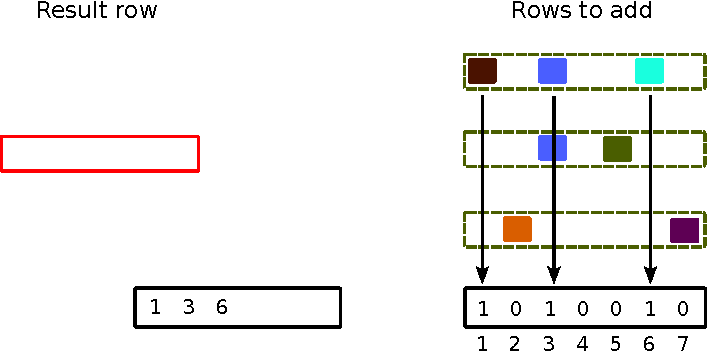
\includegraphics[width=0.7\textwidth]{figures/spgemm-sorted-6} }\only<7>{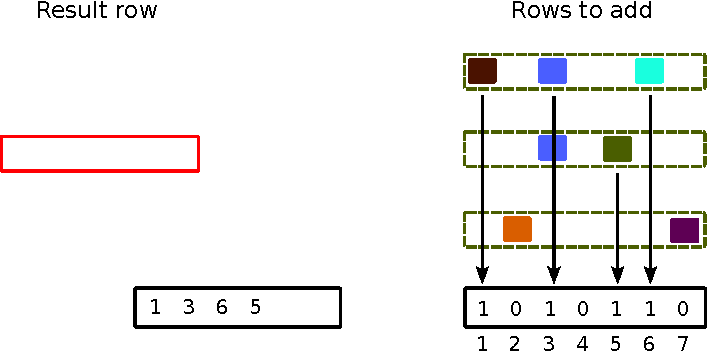
\includegraphics[width=0.7\textwidth]{figures/spgemm-sorted-7} }\only<8>{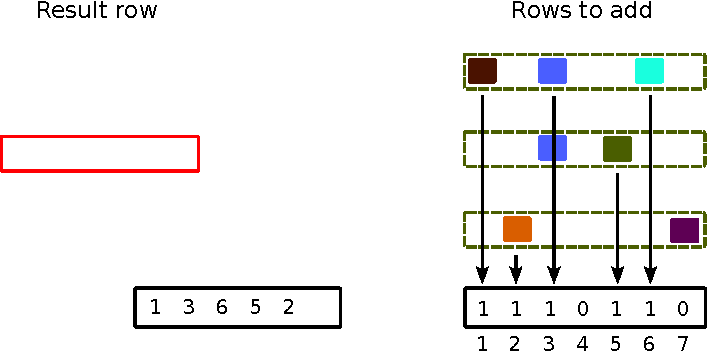
\includegraphics[width=0.7\textwidth]{figures/spgemm-sorted-8} }\only<9>{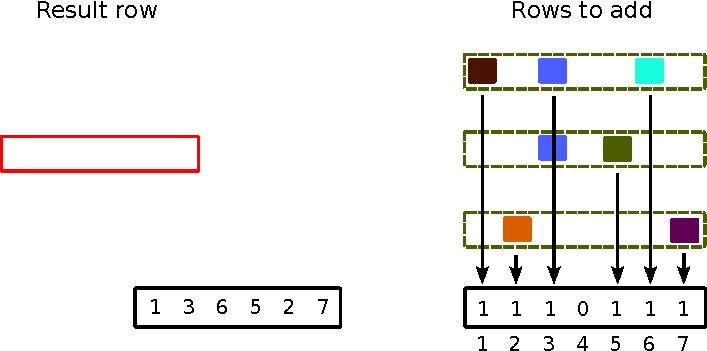
\includegraphics[width=0.7\textwidth]{figures/spgemm-sorted-9} }\only<10>{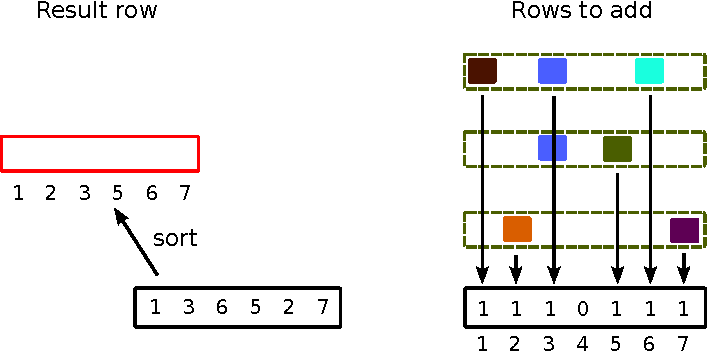
\includegraphics[width=0.7\textwidth]{figures/spgemm-sorted-10} }
\end{center}

 \begin{block}{Sorted MatMatMult in PETSc}
  \begin{itemize}
   \item Dense flag array
   \item Segmented buffer for nonzero indices
  \end{itemize}
 \end{block}

\end{frame}


\begin{frame}{Sparse Matrix-Matrix Multiplications}

\begin{center}
\only<1>{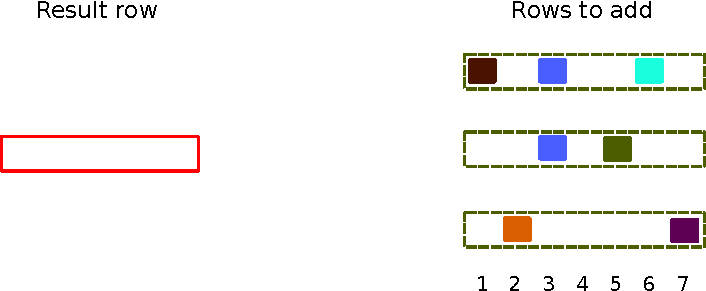
\includegraphics[width=0.7\textwidth]{figures/spgemm-scalable-2} }\only<2>{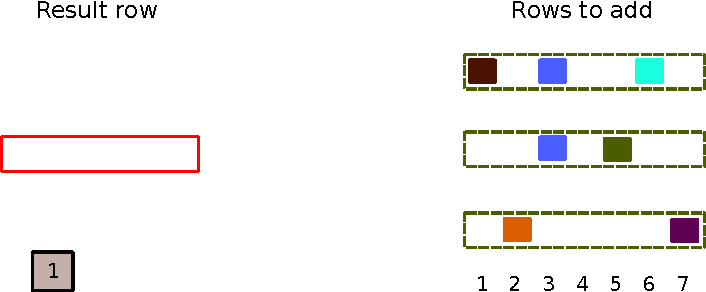
\includegraphics[width=0.7\textwidth]{figures/spgemm-scalable-3} }\only<3>{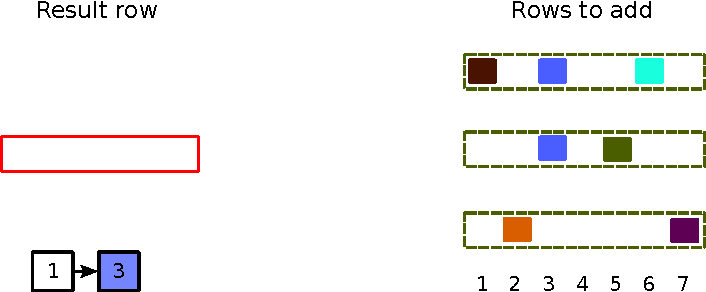
\includegraphics[width=0.7\textwidth]{figures/spgemm-scalable-4} }\only<4>{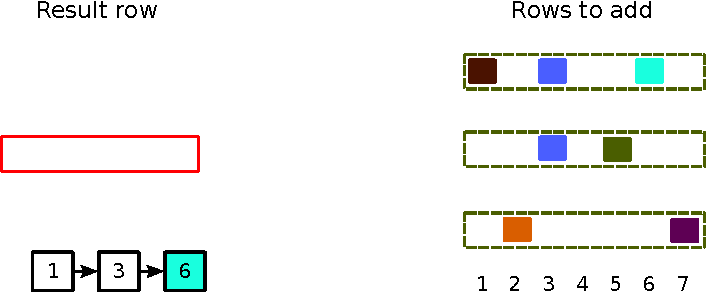
\includegraphics[width=0.7\textwidth]{figures/spgemm-scalable-5} }\only<5>{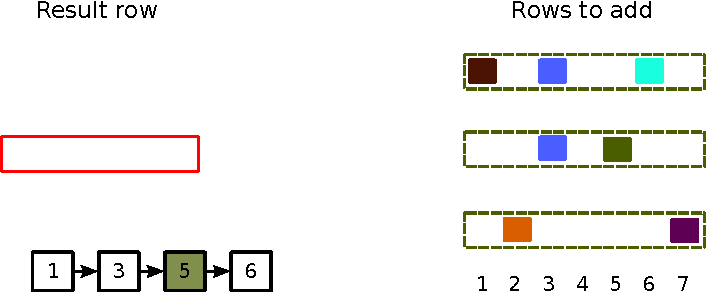
\includegraphics[width=0.7\textwidth]{figures/spgemm-scalable-6} }\only<6>{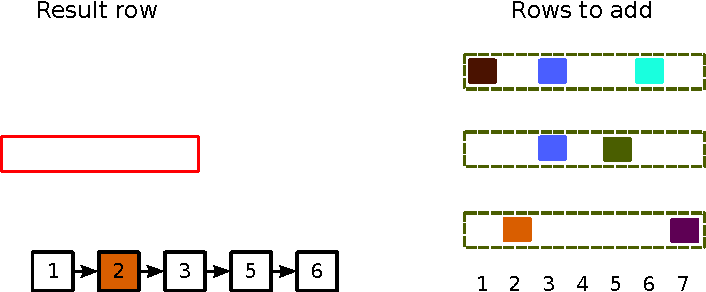
\includegraphics[width=0.7\textwidth]{figures/spgemm-scalable-7} }\only<7>{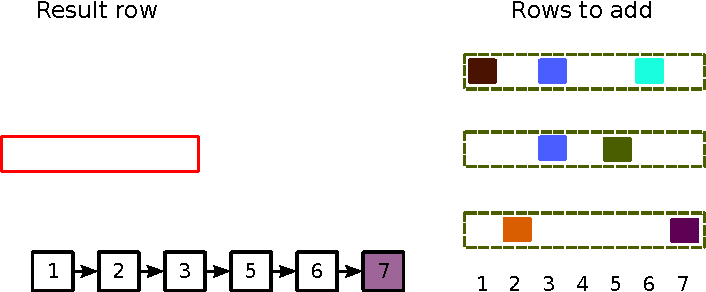
\includegraphics[width=0.7\textwidth]{figures/spgemm-scalable-8} }\only<8>{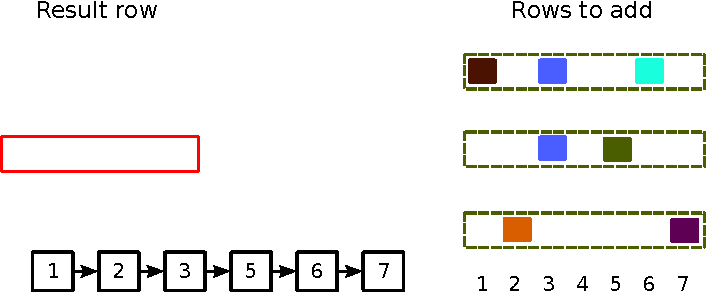
\includegraphics[width=0.7\textwidth]{figures/spgemm-scalable-9} }\only<9>{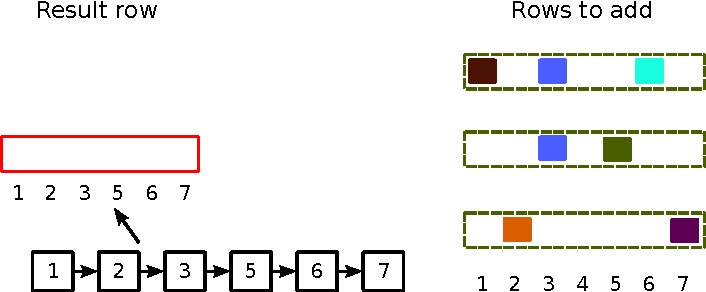
\includegraphics[width=0.7\textwidth]{figures/spgemm-scalable-10} }
\end{center}

 \begin{block}{Scalable MatMatMult in PETSc}
  \begin{itemize}
   \visible<2->{\item Use \{linked list, heap, binary tree\} to merge nonzero column indices}
   \visible<2->{\item No dense array}
  \end{itemize}
 \end{block}

\end{frame}





%%
%% Algorithm
%%



%%
%% Algorithm
%%


\begin{frame}{Row Merge Algorithm}

\begin{center}
\only<1>{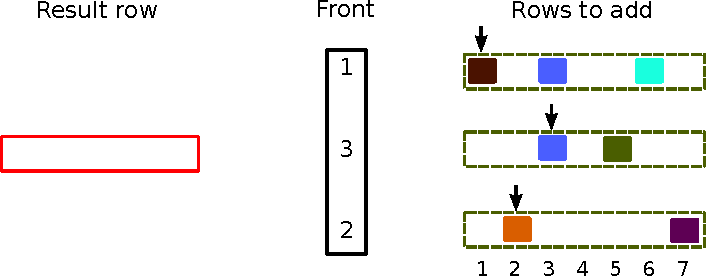
\includegraphics[width=0.7\textwidth]{figures/spgemm-row-0} }\only<2>{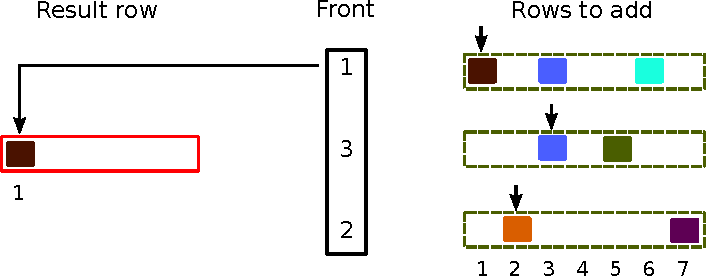
\includegraphics[width=0.7\textwidth]{figures/spgemm-row-1} }\only<3>{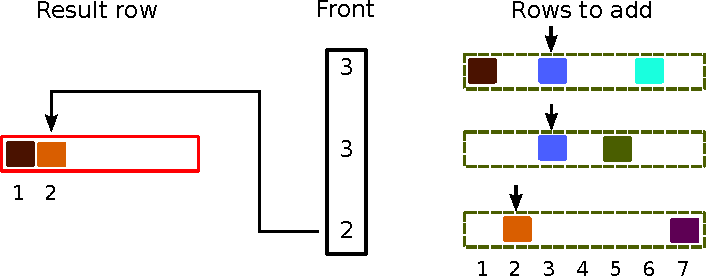
\includegraphics[width=0.7\textwidth]{figures/spgemm-row-2} }\only<4>{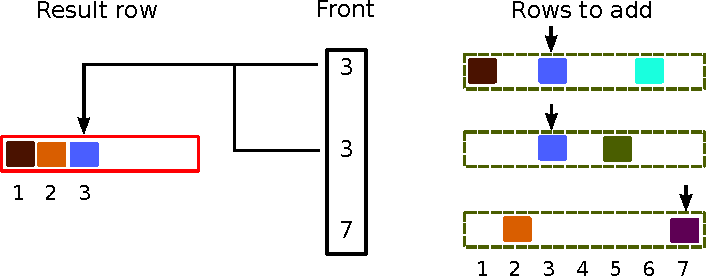
\includegraphics[width=0.7\textwidth]{figures/spgemm-row-3} }\only<5>{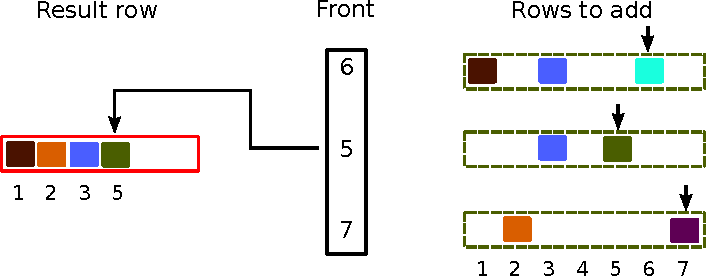
\includegraphics[width=0.7\textwidth]{figures/spgemm-row-4} }\only<6>{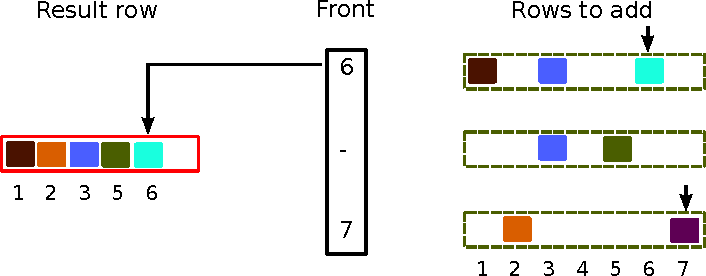
\includegraphics[width=0.7\textwidth]{figures/spgemm-row-5} }\only<7>{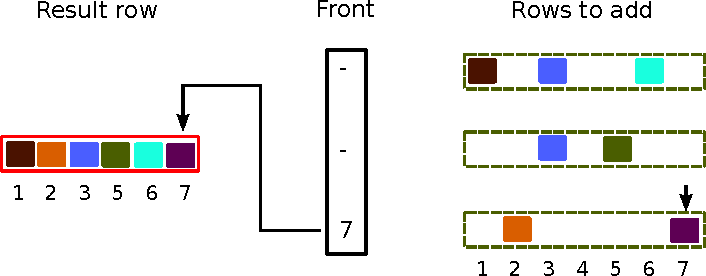
\includegraphics[width=0.7\textwidth]{figures/spgemm-row-6} }
\end{center}


\begin{block}{Result Row Computation}
 \begin{enumerate}
  \item Determine minimum index in front
  \pause
  \item Write minimum index
  \pause
  \item Advance front where minimum index occurred
 \end{enumerate}

\end{block}


\end{frame}

%%%%%%%%%%%


\begin{frame}[fragile]{Sparse Matrix Products}

 \begin{minipage}{0.44\textwidth}
 \begin{block}{Algorithm Details}
  \begin{itemize}
   \item Split matrix if rows too large
   \item Recursively merge 8 rows
   \item (Re-)use scratchpad memory
  \end{itemize}
 \end{block}
 \end{minipage}
 \begin{minipage}{0.55\textwidth}
  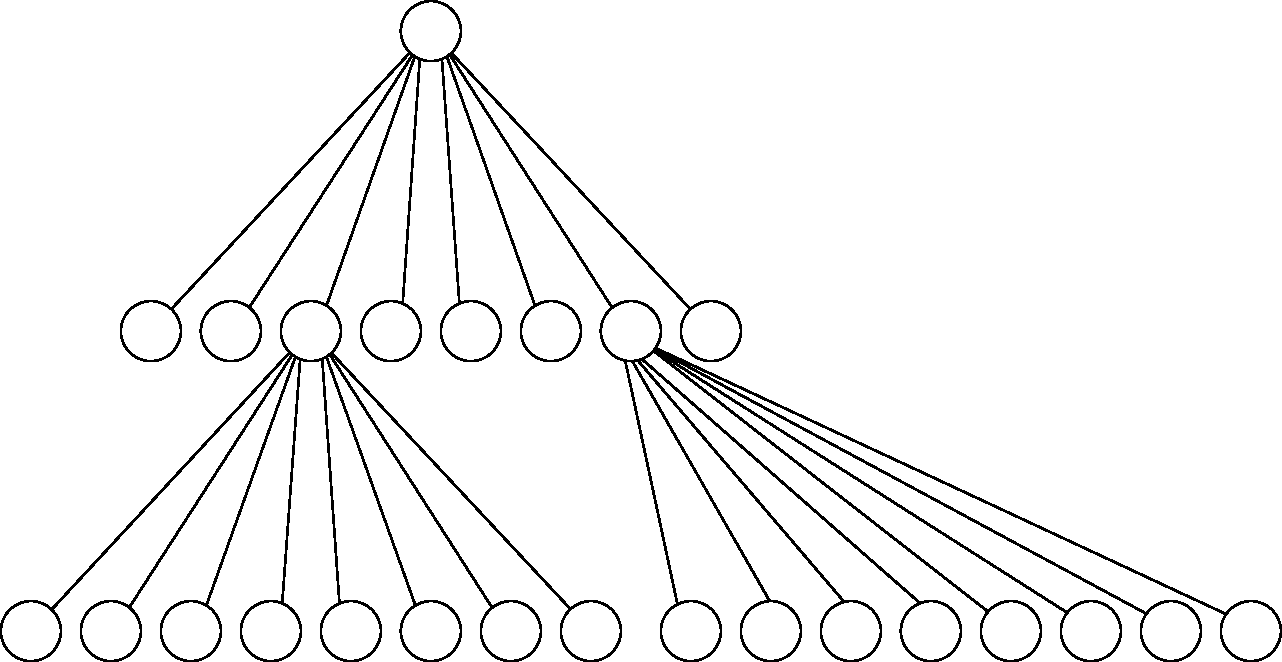
\includegraphics[width=0.999\textwidth]{figures/Octree2} \\
  {\tiny \verb|https://en.wikipedia.org/wiki/Octree\#/media/File:Octree2.svg|}
 \end{minipage}

 \pause
 \begin{block}{Hardware Details}
  \begin{itemize}
   \item CPU: Use AVX2 to merge 8 rows simultaneously
   \item GPU: Merge up to 32/64 rows simultaneously with one warp/wavefront
   \item MIC: Use AVX-KNC to merge 16 rows simultaneously
  \end{itemize}
 \end{block}

 \pause
  \begin{block}{Parallelization and Load Balancing}
  \begin{itemize}
   \item CPU, MIC: Use MPI!
   \item CPU, MIC, alternative: OpenMP dynamic scheduling, chunk size 1024
   \item GPU: thread scheduling in hardware
  \end{itemize}
 \end{block}


\end{frame}




%%
%% Benchmarks
%%




%\begin{frame}{Benchmarks}
%  \begin{center}
%   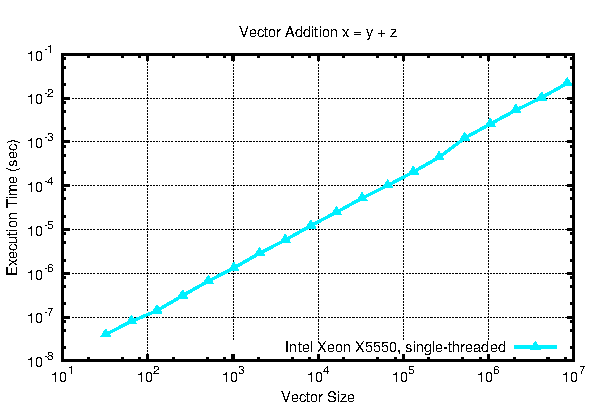
\includegraphics[width=0.95\textwidth]{figures/vector-timings-1}
%  \end{center}
%\end{frame}

%\begin{frame}{Benchmarks}
%  \begin{center}
%   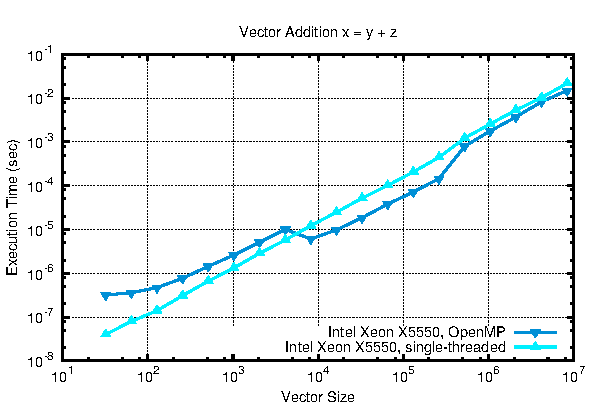
\includegraphics[width=0.95\textwidth]{figures/vector-timings-2}
%  \end{center}
%\end{frame}

%\begin{frame}{Benchmarks}
%  \begin{center}
%   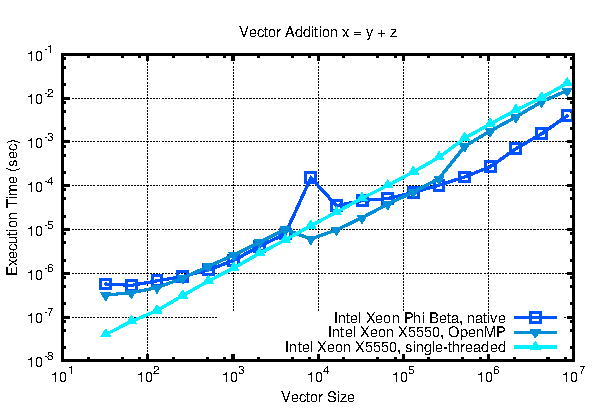
\includegraphics[width=0.95\textwidth]{figures/vector-timings-3}
%  \end{center}
%\end{frame}

%\begin{frame}{Benchmarks}
%  \begin{center}
%   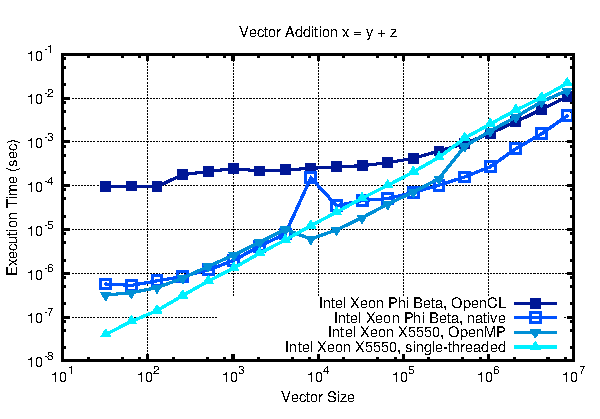
\includegraphics[width=0.95\textwidth]{figures/vector-timings-4}
%  \end{center}
%\end{frame}

%\begin{frame}{Benchmarks}
%  \begin{center}
%   \includegraphics[width=0.95\textwidth]{figures/vector-timings-5}
%  \end{center}
%\end{frame}

%\begin{frame}{Benchmarks}
%  \begin{center}
%   \includegraphics[width=0.95\textwidth]{figures/vector-timings-6}
%  \end{center}
%\end{frame}

\begin{frame}{Benchmarks}
  \begin{center}
   \includegraphics[width=0.95\textwidth]{figures/vector-timings-7}
  \end{center}
\end{frame}

%%

%\begin{frame}{Benchmarks}
%  \begin{center}
%   \includegraphics[width=0.95\textwidth]{figures/cg-timings-1}
%  \end{center}
%\end{frame}

%\begin{frame}{Benchmarks}
%  \begin{center}
%   \includegraphics[width=0.95\textwidth]{figures/cg-timings-2}
%  \end{center}
%\end{frame}

%\begin{frame}{Benchmarks}
%  \begin{center}
%   \includegraphics[width=0.95\textwidth]{figures/cg-timings-3}
%  \end{center}
%\end{frame}

%\begin{frame}{Benchmarks}
%  \begin{center}
%   \includegraphics[width=0.95\textwidth]{figures/cg-timings-4}
%  \end{center}
%\end{frame}

%\begin{frame}{Benchmarks}
%  \begin{center}
%   \includegraphics[width=0.95\textwidth]{figures/cg-timings-5}
%  \end{center}
%\end{frame}

%\begin{frame}{Benchmarks}
%  \begin{center}
%   \includegraphics[width=0.95\textwidth]{figures/cg-timings-6}
%  \end{center}
%\end{frame}

\begin{frame}{Benchmarks}
  \begin{center}
   \includegraphics[width=0.95\textwidth]{figures/cg-timings-7}
  \end{center}
\end{frame}


\begin{frame}{Benchmarks}

 \begin{block}{Matrix-Matrix Multiplication}
  \begin{itemize}
   \item Autotuning environment 
   \item \includegraphics[width=0.85\textwidth]{figures/gemm3.pdf}
   \item \centering (AMD Radeon HD 7970, single precision)
  \end{itemize}

 \end{block}

\end{frame}






%%
%% Distributed SpGEMM
%%



\begin{frame}{Sparse Matrix-Matrix Multiplications}

 \begin{block}{Parallel MatMatMult in PETSc}
  \begin{itemize}
   \item Scalable
   \item Non-Scalable
  \end{itemize}
 \end{block}

\begin{center}
\only<1>{\includegraphics[width=0.9\textwidth]{figures/spgemm-parallel-1} }\only<2>{\includegraphics[width=0.9\textwidth]{figures/spgemm-parallel-2} }\only<3->{\includegraphics[width=0.9\textwidth]{figures/spgemm-parallel-3} }
\end{center}

\visible<4>{
\vspace*{.5cm}
\begin{center}
  {\Large \textbf{Lots of bookkeeping...} }
\end{center}
}

\end{frame}







%%
%% Summary
%%

\begin{frame}{Summary}

 \begin{block}{Sequential Sparse Matrix-Matrix Products}
   \begin{itemize}
    \item Row Merge faster than MKL on Xeon CPUs on average
    \item Row Merge faster than cuSPARSE and CUSP on Tesla K20m (and others)
   \end{itemize}
 \end{block}

 \pause
  \begin{block}{Parallel Sparse Matrix-Matrix Products}
   \begin{itemize}
    \item Potential for an approach similar to Row Merge
    \item Fine-tune use of scalable vs.~non-scalable routines
   \end{itemize}
 \end{block}

 \pause
 \begin{block}{Implications and Outlook}
   \begin{itemize}
    \item CPUs beat accelerators for sparse matrix-matrix products (caches!)
    \item Full integration into PETSc's GAMG (algebraic multigrid)
    \item Find CPU/GPU balance for hybrid clusters
   \end{itemize}
 \end{block}

\end{frame}



\end{document}

